\documentclass[]{elsarticle} %review=doublespace preprint=single 5p=2 column
%%% Begin My package additions %%%%%%%%%%%%%%%%%%%
\usepackage[hyphens]{url}

  \journal{An awesome journal} % Sets Journal name


\usepackage{lineno} % add
\providecommand{\tightlist}{%
  \setlength{\itemsep}{0pt}\setlength{\parskip}{0pt}}

\usepackage{graphicx}
\usepackage{booktabs} % book-quality tables
%%%%%%%%%%%%%%%% end my additions to header

\usepackage[T1]{fontenc}
\usepackage{lmodern}
\usepackage{amssymb,amsmath}
\usepackage{ifxetex,ifluatex}
\usepackage{fixltx2e} % provides \textsubscript
% use upquote if available, for straight quotes in verbatim environments
\IfFileExists{upquote.sty}{\usepackage{upquote}}{}
\ifnum 0\ifxetex 1\fi\ifluatex 1\fi=0 % if pdftex
  \usepackage[utf8]{inputenc}
\else % if luatex or xelatex
  \usepackage{fontspec}
  \ifxetex
    \usepackage{xltxtra,xunicode}
  \fi
  \defaultfontfeatures{Mapping=tex-text,Scale=MatchLowercase}
  \newcommand{\euro}{€}
\fi
% use microtype if available
\IfFileExists{microtype.sty}{\usepackage{microtype}}{}
\bibliographystyle{elsarticle-harv}
\usepackage{graphicx}
\ifxetex
  \usepackage[setpagesize=false, % page size defined by xetex
              unicode=false, % unicode breaks when used with xetex
              xetex]{hyperref}
\else
  \usepackage[unicode=true]{hyperref}
\fi
\hypersetup{breaklinks=true,
            bookmarks=true,
            pdfauthor={},
            pdftitle={Rpackage for the automatic estimation of the parameters of the Von Bertalanffy fish growth model},
            colorlinks=false,
            urlcolor=blue,
            linkcolor=magenta,
            pdfborder={0 0 0}}
\urlstyle{same}  % don't use monospace font for urls

\setcounter{secnumdepth}{0}
% Pandoc toggle for numbering sections (defaults to be off)
\setcounter{secnumdepth}{0}

% Pandoc citation processing

% Pandoc header



\begin{document}
\begin{frontmatter}

  \title{Rpackage for the automatic estimation of the parameters of the Von
Bertalanffy fish growth model}
    \author[Université de Lille]{Marine Ballutaud\corref{1}}
   \ead{marine.ballutaud@univ-lille.fr} 
    \author[IFREMER]{Lyndsay Clavareau\corref{2}}
   \ead{lyndsay.clavareau@ifremer.fr} 
    \author[Observatoire Pelagis]{Etienne Rouby\corref{2}}
   \ead{etienne.rouby@univ-lr.fr} 
    \author[Centre d'Ecologie Fonctionnelle et Evolutive]{Julien Renoult\corref{2}}
   \ead{julien.renoult@blabla.com} 
    \author[Cirad]{Fabienne Ribeyre\corref{2}}
   \ead{fabienne.ribeyre@cirad.fr} 
      \address[Université de Lille]{Department, Street, City, State, Zip}
      \cortext[1]{Corresponding Author}
    \cortext[2]{Equal contribution}
  
  \begin{abstract}
  This is the abstract.
  \end{abstract}
  
 \end{frontmatter}

\hypertarget{introduction}{%
\section{Introduction}\label{introduction}}

This package was created as part of the training course ``Good practices
for reproducible research in digital ecology'' co-organized by the Cesab
of the FRB and the GDR EcoStat. It uses the model de Bertalanffy (1938).

\hypertarget{material-and-methods}{%
\section{Material and methods}\label{material-and-methods}}

\hypertarget{datasource}{%
\paragraph{Datasource}\label{datasource}}

The data used comes from the website https://www.fishbase.in/home.htm.

\hypertarget{statistical-methods}{%
\paragraph{Statistical methods}\label{statistical-methods}}

The Growth model of Von Bertalanffy is \[Linf.(1-exp^{-K*(a-to)})\] with
Linf = maximum size, a = fish age, K and t0 are fixed parameters.

Model was adjusted using the method described by Rafail (1973).

\hypertarget{results}{%
\section{Results}\label{results}}

The results of the model are presented in Figure 1.

\begin{figure}
\centering
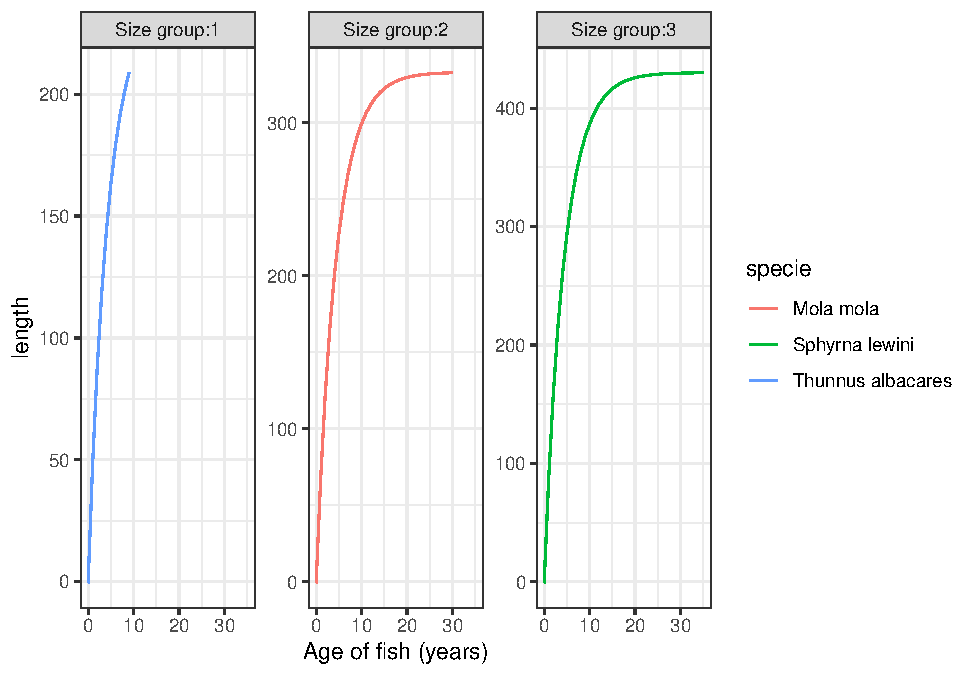
\includegraphics{ElsevierRBertalanffyPackage_files/figure-latex/unnamed-chunk-1-1.pdf}
\caption{Growth curve obtained with the Growth model of Von Bertalanffy}
\end{figure}

\hypertarget{discussion}{%
\section{Discussion}\label{discussion}}

Working with others on a project is much more complicated than working
alone, but much faster.

\hypertarget{references}{%
\section*{References}\label{references}}
\addcontentsline{toc}{section}{References}

\hypertarget{refs}{}
\leavevmode\hypertarget{ref-Bertalanffy1938}{}%
Bertalanffy, L. von, 1938. A quantitative theory of organic growth
(inquiries on growth laws ii). Human Biology 10, 181--213.

\leavevmode\hypertarget{ref-rafail_simple_1973}{}%
Rafail, S.Z., 1973. A simple and precise method for fitting a von
Bertalanffy growth curve. Marine Biology 19, 354--358.
doi:\href{https://doi.org/10.1007/BF00348907}{10.1007/BF00348907}


\end{document}


